% Options for packages loaded elsewhere
\PassOptionsToPackage{unicode}{hyperref}
\PassOptionsToPackage{hyphens}{url}
\PassOptionsToPackage{dvipsnames,svgnames,x11names}{xcolor}
%
\documentclass[
  letterpaper,
  DIV=11,
  numbers=noendperiod]{scrreprt}

\usepackage{amsmath,amssymb}
\usepackage{iftex}
\ifPDFTeX
  \usepackage[T1]{fontenc}
  \usepackage[utf8]{inputenc}
  \usepackage{textcomp} % provide euro and other symbols
\else % if luatex or xetex
  \usepackage{unicode-math}
  \defaultfontfeatures{Scale=MatchLowercase}
  \defaultfontfeatures[\rmfamily]{Ligatures=TeX,Scale=1}
\fi
\usepackage{lmodern}
\ifPDFTeX\else  
    % xetex/luatex font selection
\fi
% Use upquote if available, for straight quotes in verbatim environments
\IfFileExists{upquote.sty}{\usepackage{upquote}}{}
\IfFileExists{microtype.sty}{% use microtype if available
  \usepackage[]{microtype}
  \UseMicrotypeSet[protrusion]{basicmath} % disable protrusion for tt fonts
}{}
\makeatletter
\@ifundefined{KOMAClassName}{% if non-KOMA class
  \IfFileExists{parskip.sty}{%
    \usepackage{parskip}
  }{% else
    \setlength{\parindent}{0pt}
    \setlength{\parskip}{6pt plus 2pt minus 1pt}}
}{% if KOMA class
  \KOMAoptions{parskip=half}}
\makeatother
\usepackage{xcolor}
\setlength{\emergencystretch}{3em} % prevent overfull lines
\setcounter{secnumdepth}{5}
% Make \paragraph and \subparagraph free-standing
\ifx\paragraph\undefined\else
  \let\oldparagraph\paragraph
  \renewcommand{\paragraph}[1]{\oldparagraph{#1}\mbox{}}
\fi
\ifx\subparagraph\undefined\else
  \let\oldsubparagraph\subparagraph
  \renewcommand{\subparagraph}[1]{\oldsubparagraph{#1}\mbox{}}
\fi

\usepackage{color}
\usepackage{fancyvrb}
\newcommand{\VerbBar}{|}
\newcommand{\VERB}{\Verb[commandchars=\\\{\}]}
\DefineVerbatimEnvironment{Highlighting}{Verbatim}{commandchars=\\\{\}}
% Add ',fontsize=\small' for more characters per line
\usepackage{framed}
\definecolor{shadecolor}{RGB}{241,243,245}
\newenvironment{Shaded}{\begin{snugshade}}{\end{snugshade}}
\newcommand{\AlertTok}[1]{\textcolor[rgb]{0.68,0.00,0.00}{#1}}
\newcommand{\AnnotationTok}[1]{\textcolor[rgb]{0.37,0.37,0.37}{#1}}
\newcommand{\AttributeTok}[1]{\textcolor[rgb]{0.40,0.45,0.13}{#1}}
\newcommand{\BaseNTok}[1]{\textcolor[rgb]{0.68,0.00,0.00}{#1}}
\newcommand{\BuiltInTok}[1]{\textcolor[rgb]{0.00,0.23,0.31}{#1}}
\newcommand{\CharTok}[1]{\textcolor[rgb]{0.13,0.47,0.30}{#1}}
\newcommand{\CommentTok}[1]{\textcolor[rgb]{0.37,0.37,0.37}{#1}}
\newcommand{\CommentVarTok}[1]{\textcolor[rgb]{0.37,0.37,0.37}{\textit{#1}}}
\newcommand{\ConstantTok}[1]{\textcolor[rgb]{0.56,0.35,0.01}{#1}}
\newcommand{\ControlFlowTok}[1]{\textcolor[rgb]{0.00,0.23,0.31}{#1}}
\newcommand{\DataTypeTok}[1]{\textcolor[rgb]{0.68,0.00,0.00}{#1}}
\newcommand{\DecValTok}[1]{\textcolor[rgb]{0.68,0.00,0.00}{#1}}
\newcommand{\DocumentationTok}[1]{\textcolor[rgb]{0.37,0.37,0.37}{\textit{#1}}}
\newcommand{\ErrorTok}[1]{\textcolor[rgb]{0.68,0.00,0.00}{#1}}
\newcommand{\ExtensionTok}[1]{\textcolor[rgb]{0.00,0.23,0.31}{#1}}
\newcommand{\FloatTok}[1]{\textcolor[rgb]{0.68,0.00,0.00}{#1}}
\newcommand{\FunctionTok}[1]{\textcolor[rgb]{0.28,0.35,0.67}{#1}}
\newcommand{\ImportTok}[1]{\textcolor[rgb]{0.00,0.46,0.62}{#1}}
\newcommand{\InformationTok}[1]{\textcolor[rgb]{0.37,0.37,0.37}{#1}}
\newcommand{\KeywordTok}[1]{\textcolor[rgb]{0.00,0.23,0.31}{#1}}
\newcommand{\NormalTok}[1]{\textcolor[rgb]{0.00,0.23,0.31}{#1}}
\newcommand{\OperatorTok}[1]{\textcolor[rgb]{0.37,0.37,0.37}{#1}}
\newcommand{\OtherTok}[1]{\textcolor[rgb]{0.00,0.23,0.31}{#1}}
\newcommand{\PreprocessorTok}[1]{\textcolor[rgb]{0.68,0.00,0.00}{#1}}
\newcommand{\RegionMarkerTok}[1]{\textcolor[rgb]{0.00,0.23,0.31}{#1}}
\newcommand{\SpecialCharTok}[1]{\textcolor[rgb]{0.37,0.37,0.37}{#1}}
\newcommand{\SpecialStringTok}[1]{\textcolor[rgb]{0.13,0.47,0.30}{#1}}
\newcommand{\StringTok}[1]{\textcolor[rgb]{0.13,0.47,0.30}{#1}}
\newcommand{\VariableTok}[1]{\textcolor[rgb]{0.07,0.07,0.07}{#1}}
\newcommand{\VerbatimStringTok}[1]{\textcolor[rgb]{0.13,0.47,0.30}{#1}}
\newcommand{\WarningTok}[1]{\textcolor[rgb]{0.37,0.37,0.37}{\textit{#1}}}

\providecommand{\tightlist}{%
  \setlength{\itemsep}{0pt}\setlength{\parskip}{0pt}}\usepackage{longtable,booktabs,array}
\usepackage{calc} % for calculating minipage widths
% Correct order of tables after \paragraph or \subparagraph
\usepackage{etoolbox}
\makeatletter
\patchcmd\longtable{\par}{\if@noskipsec\mbox{}\fi\par}{}{}
\makeatother
% Allow footnotes in longtable head/foot
\IfFileExists{footnotehyper.sty}{\usepackage{footnotehyper}}{\usepackage{footnote}}
\makesavenoteenv{longtable}
\usepackage{graphicx}
\makeatletter
\def\maxwidth{\ifdim\Gin@nat@width>\linewidth\linewidth\else\Gin@nat@width\fi}
\def\maxheight{\ifdim\Gin@nat@height>\textheight\textheight\else\Gin@nat@height\fi}
\makeatother
% Scale images if necessary, so that they will not overflow the page
% margins by default, and it is still possible to overwrite the defaults
% using explicit options in \includegraphics[width, height, ...]{}
\setkeys{Gin}{width=\maxwidth,height=\maxheight,keepaspectratio}
% Set default figure placement to htbp
\makeatletter
\def\fps@figure{htbp}
\makeatother

\KOMAoption{captions}{tableheading}
\makeatletter
\@ifpackageloaded{bookmark}{}{\usepackage{bookmark}}
\makeatother
\makeatletter
\@ifpackageloaded{caption}{}{\usepackage{caption}}
\AtBeginDocument{%
\ifdefined\contentsname
  \renewcommand*\contentsname{Table of contents}
\else
  \newcommand\contentsname{Table of contents}
\fi
\ifdefined\listfigurename
  \renewcommand*\listfigurename{List of Figures}
\else
  \newcommand\listfigurename{List of Figures}
\fi
\ifdefined\listtablename
  \renewcommand*\listtablename{List of Tables}
\else
  \newcommand\listtablename{List of Tables}
\fi
\ifdefined\figurename
  \renewcommand*\figurename{Figure}
\else
  \newcommand\figurename{Figure}
\fi
\ifdefined\tablename
  \renewcommand*\tablename{Table}
\else
  \newcommand\tablename{Table}
\fi
}
\@ifpackageloaded{float}{}{\usepackage{float}}
\floatstyle{ruled}
\@ifundefined{c@chapter}{\newfloat{codelisting}{h}{lop}}{\newfloat{codelisting}{h}{lop}[chapter]}
\floatname{codelisting}{Listing}
\newcommand*\listoflistings{\listof{codelisting}{List of Listings}}
\makeatother
\makeatletter
\makeatother
\makeatletter
\@ifpackageloaded{caption}{}{\usepackage{caption}}
\@ifpackageloaded{subcaption}{}{\usepackage{subcaption}}
\makeatother
\ifLuaTeX
  \usepackage{selnolig}  % disable illegal ligatures
\fi
\usepackage{bookmark}

\IfFileExists{xurl.sty}{\usepackage{xurl}}{} % add URL line breaks if available
\urlstyle{same} % disable monospaced font for URLs
\hypersetup{
  pdftitle={Value Chain Hackers - Documentation},
  pdfauthor={Christiaan Verhoef},
  colorlinks=true,
  linkcolor={blue},
  filecolor={Maroon},
  citecolor={Blue},
  urlcolor={Blue},
  pdfcreator={LaTeX via pandoc}}

\title{Value Chain Hackers - Documentation}
\author{Christiaan Verhoef}
\date{2026-03-06}

\begin{document}
\maketitle

\renewcommand*\contentsname{Table of contents}
{
\hypersetup{linkcolor=}
\setcounter{tocdepth}{2}
\tableofcontents
}
\bookmarksetup{startatroot}

\chapter{Welcome to Value Chain
Hackers}\label{welcome-to-value-chain-hackers}

\bookmarksetup{startatroot}

\chapter{Welcome}\label{welcome}

Hello and a warm welcome to the Value Chain Hackers onboarding
documentation! I'm Christiaan Verhoef, your guide, mentor, and fellow
enthusiast in this exciting journey. Whether you're a student, mentor,
or project manager, this guide is here to provide you with all the tools
and insights you need to thrive in our vibrant community.

\section{Our Mission}\label{our-mission}

At Value Chain Hackers, we are on a mission to revolutionize the supply
chain industry through relentless innovation, spirited collaboration,
and hands-on practical application. We believe in empowering each
individual to make meaningful contributions that drive real-world
impact. Together, we will tackle the complexities of supply chains and
transform challenges into opportunities.

\section{What to Expect}\label{what-to-expect}

Over the next 16 weeks, you'll dive into an immersive program designed
to challenge your skills, broaden your horizons, and foster strong team
dynamics. Here's a glimpse of what lies ahead:

\begin{itemize}
\tightlist
\item
  \textbf{Kick-off Hackathon}: Begin with an exhilarating one-day
  hackathon where you'll meet your team, brainstorm groundbreaking
  ideas, and set the stage for an unforgettable semester.
\item
  \textbf{Bi-Weekly SCRUM Meetings}: Engage in regular check-ins to
  discuss progress, overcome obstacles, and ensure we are all aligned
  with our project goals.
\item
  \textbf{Mentorship and Support}: Gain from the wisdom and experience
  of our dedicated mentors, who will act as your patrons, guiding you
  every step of the way.
\item
  \textbf{Hands-On Projects}: Work on real-world supply chain problems,
  applying your skills and creativity to develop innovative solutions
  that make a difference.
\item
  \textbf{Celebration and Recognition}: Conclude the semester with a
  grand closing ceremony where you'll showcase your findings, share your
  experiences, and celebrate your achievements together.
\end{itemize}

\section{Getting Started}\label{getting-started}

\begin{enumerate}
\def\labelenumi{\arabic{enumi}.}
\tightlist
\item
  \textbf{Read the Documentation}: Dive into the program structure,
  roles, and responsibilities by reading through this comprehensive
  documentation.
\item
  \textbf{Join Our Communication Channels}: Connect with your peers and
  mentors on Discord and stay updated with official announcements via
  Nextcloud.
\item
  \textbf{Set Up Your Tools}: Ensure you have access to all necessary
  tools, including Taiga for project management, GitLab for version
  control, and Jitsi for virtual meetings.
\item
  \textbf{Participate Actively}: Immerse yourself in all scheduled
  activities, contribute to discussions, and collaborate with your team
  to maximize this learning experience.
\end{enumerate}

\section{Contact Information}\label{contact-information}

If you have any questions or need assistance, don't hesitate to reach
out:

\begin{itemize}
\tightlist
\item
  \textbf{Email}:
  \href{mailto:cg.verhoef@windesheim.nl}{\nolinkurl{cg.verhoef@windesheim.nl}}
\item
  \textbf{Discord}: Join our server
  \href{https://discord.gg/zzA7YSsY}{here}
\end{itemize}

\section{Conclusion}\label{conclusion}

We are thrilled to have you on board and cannot wait to witness the
amazing things you'll achieve as part of the Value Chain Hackers
program. Together, let's embark on this transformative journey and make
a lasting impact in the world of supply chain management!

Welcome to the team!

Christiaan Verhoef\\
Value Chain Hackers Leader

\bookmarksetup{startatroot}

\chapter{Introduction}\label{introduction}

\bookmarksetup{startatroot}

\chapter{Introduction}\label{introduction-1}

Welcome to the Value Chain Hackers! In this program, you will embark on
an exciting journey to revolutionize the supply chain industry through
innovation, collaboration, and practical application. Our goal is to
equip you with the tools, knowledge, and support you need to make
meaningful contributions and drive real-world impact.

Throughout this program, you'll be challenged to think critically, work
collaboratively, and apply your skills to solve complex supply chain
problems. You'll have the opportunity to learn from experienced mentors,
engage with industry experts, and collaborate with peers who share your
passion for innovation.

Get ready to dive into a dynamic and immersive experience that will push
your boundaries, expand your horizons, and prepare you to become a
leader in the supply chain industry. Together, we'll transform
challenges into opportunities and create a brighter future for supply
chain management.

\section{Inspiring Videos}\label{inspiring-videos}

To kickstart your journey, here are some inspiring videos that explore
themes related to supply chains, innovation, and teamwork. These videos
highlight the power of creativity, resilience, and collaboration in
overcoming challenges and achieving success:

\subsection{How Wolves Change Rivers}\label{how-wolves-change-rivers}

An incredible story about how the reintroduction of wolves to
Yellowstone National Park changed the entire ecosystem, illustrating the
powerful impact of a single change in a system.

\begin{figure}[H]

{\centering 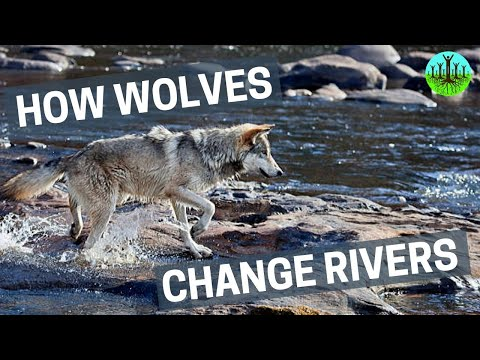
\includegraphics{index_files/mediabag/0.jpg}

}

\caption{How Wolves Change Rivers}

\end{figure}%

\subsection{Simon Sinek: How Great Leaders Inspire
Action}\label{simon-sinek-how-great-leaders-inspire-action}

Simon Sinek discusses the concept of ``Start With Why'' and how leaders
inspire action by focusing on their purpose and values.

\begin{figure}[H]

{\centering 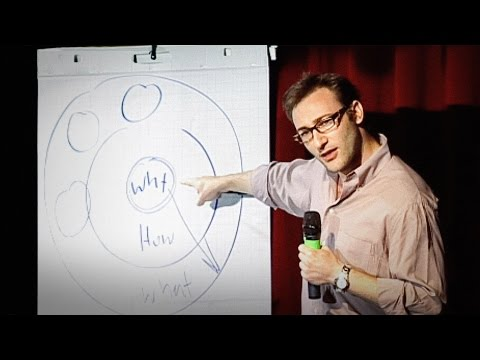
\includegraphics{index_files/mediabag/01.jpg}

}

\caption{How Great Leaders Inspire Action}

\end{figure}%

\subsection{RSA ANIMATE: Drive: The surprising truth about what
motivates
us}\label{rsa-animate-drive-the-surprising-truth-about-what-motivates-us}

An animated version of Dan Pink's talk on motivation, exploring the
science behind what drives us to work harder and be more creative.

\begin{figure}[H]

{\centering 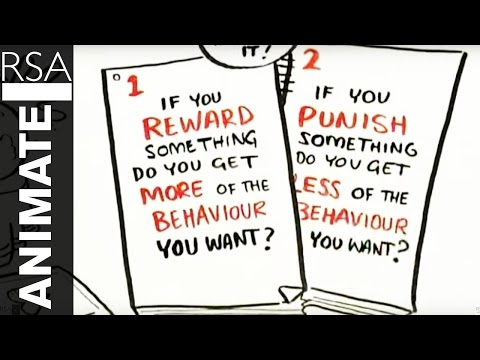
\includegraphics{index_files/mediabag/012.jpg}

}

\caption{Drive: The surprising truth about what motivates us}

\end{figure}%

\subsection{The Power of Vulnerability - Brené
Brown}\label{the-power-of-vulnerability---brenuxe9-brown}

Brené Brown shares her research on vulnerability, highlighting its
importance in fostering innovation, creativity, and change.

\begin{figure}[H]

{\centering 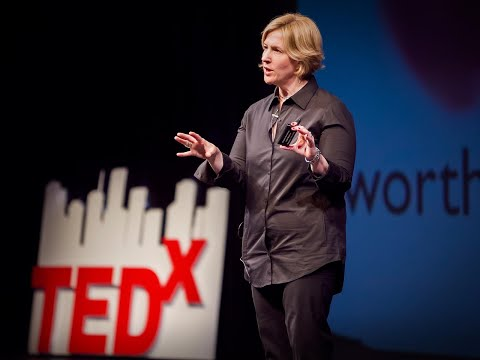
\includegraphics{index_files/mediabag/0123.jpg}

}

\caption{The Power of Vulnerability}

\end{figure}%

These videos will not only inspire you but also provide valuable
insights into innovation, resilience, and the power of teamwork. Enjoy
watching them as you embark on your Value Chain Hackers journey!

Let's get started!

\bookmarksetup{startatroot}

\chapter{Why}\label{why}

\bookmarksetup{startatroot}

\chapter{Why}\label{why-1}

\section{Why Value Chain Hackers}\label{why-value-chain-hackers}

Welcome to Value Chain Hackers! We are on a mission to revolutionize the
supply chain industry through innovation, collaboration, and practical
application. By providing you with the necessary resources and building
strong, agile teams, we ensure that our participants can make meaningful
contributions to the field of supply chain management. Together, we'll
tackle the complexities of supply chains and transform challenges into
opportunities.

\subsection{Unleashing Your Potential}\label{unleashing-your-potential}

Our program is all about unlocking your potential. We believe that every
participant has unique strengths and talents that, when harnessed, can
lead to extraordinary results. Through Value Chain Hackers, you'll have
the opportunity to discover and develop your abilities in a supportive
and dynamic environment.

\subsection{Real-World Impact}\label{real-world-impact}

We're not just playing around here---our goal is to make a real
difference in the world. The supply chain industry is vast and complex,
playing a crucial role in our daily lives. By improving supply chains,
we can enhance efficiency, reduce waste, and create more sustainable
practices. Your work here can lead to tangible, positive changes in the
industry and beyond.

\subsection{Innovation and Creativity}\label{innovation-and-creativity}

Innovation is at the heart of everything we do. We encourage you to
think outside the box, experiment with new ideas, and push the
boundaries of what's possible. This is your chance to bring fresh
perspectives to the table and come up with creative solutions to
challenging problems. Let's have fun with it and see where our
imagination can take us!

\subsection{Collaboration and
Community}\label{collaboration-and-community}

One of the best parts of Value Chain Hackers is the sense of community.
You'll be working alongside passionate individuals who are just as
excited about supply chain innovation as you are. Together, we'll build
a collaborative environment where ideas can flow freely, and everyone's
contributions are valued. Whether it's through brainstorming sessions,
hackathons, or casual chats over coffee, you'll find that the power of
teamwork can lead to amazing breakthroughs.

\section{Why Online Learning \& Digital
Lab}\label{why-online-learning-digital-lab}

\subsection{Flexibility and
Accessibility}\label{flexibility-and-accessibility}

The digital lab provides unparalleled flexibility and accessibility. No
matter where you are in the world, you can participate in our program.
This allows us to bring together a diverse group of individuals,
fostering a rich environment of different perspectives and ideas. Online
learning means you can fit your participation around other commitments,
ensuring you can engage fully without sacrificing other important
aspects of your life.

\subsection{Cutting-Edge Tools and
Resources}\label{cutting-edge-tools-and-resources}

By leveraging digital platforms, we provide access to a range of
cutting-edge tools and resources. From project management software like
Taiga to collaboration tools like Nextcloud and Etherpad, you'll have
everything you need at your fingertips. These tools not only facilitate
efficient workflow but also enhance your learning experience.

\subsection{Interactive and Engaging
Content}\label{interactive-and-engaging-content}

Our online learning approach is designed to be interactive and engaging.
With virtual meetings via Jitsi, real-time document editing, and dynamic
feedback systems, you'll be actively involved in your learning process.
This keeps the experience lively and ensures that you're not just
passively consuming information.

\section{Why AI for Supply Chain}\label{why-ai-for-supply-chain}

\subsection{Enhancing Efficiency}\label{enhancing-efficiency}

AI has the power to transform supply chains by enhancing efficiency.
From predictive analytics to automated decision-making, AI tools can
help identify bottlenecks, optimize routes, and forecast demand with
greater accuracy. This leads to more efficient operations and
significant cost savings.

\subsection{Driving Innovation}\label{driving-innovation}

AI is at the forefront of technological innovation. By integrating AI
into supply chain management, we open up new possibilities for
problem-solving and process improvement. AI can analyze vast amounts of
data quickly, providing insights that would be impossible to achieve
manually. This drives innovation and helps us stay ahead of industry
trends.

\subsection{Improving Sustainability}\label{improving-sustainability}

AI can also contribute to more sustainable supply chains. By optimizing
resources and reducing waste, AI-driven solutions can help companies
achieve their sustainability goals. This is increasingly important in a
world where environmental considerations are critical to business
success.

\section{Why Scrum Agile Working
Methodology}\label{why-scrum-agile-working-methodology}

\subsection{Flexibility and
Adaptability}\label{flexibility-and-adaptability}

Scrum is all about flexibility and adaptability. In a fast-paced
industry like supply chain management, the ability to pivot quickly in
response to changing conditions is crucial. Scrum provides a framework
that allows teams to respond to changes efficiently, ensuring that
projects stay on track even when unexpected challenges arise.

\subsection{Enhancing Team
Collaboration}\label{enhancing-team-collaboration}

Scrum emphasizes teamwork and collaboration. By working in sprints and
holding regular stand-up meetings, team members stay aligned and
engaged. This fosters a collaborative environment where everyone's input
is valued, and the collective effort leads to better outcomes.

\subsection{Continuous Improvement}\label{continuous-improvement}

One of the core principles of Scrum is continuous improvement. Through
regular retrospectives, teams reflect on their processes and identify
areas for enhancement. This commitment to ongoing improvement ensures
that we are always striving to be better, delivering higher quality
results with each iteration.

\subsection{Clear Goals and
Accountability}\label{clear-goals-and-accountability}

Scrum provides clear goals and accountability. Each sprint has specific
objectives, and team members know exactly what is expected of them. This
clarity helps keep everyone focused and motivated, driving progress and
ensuring that we meet our targets effectively.

\bookmarksetup{startatroot}

\chapter{How}\label{how}

\bookmarksetup{startatroot}

\chapter{How}\label{how-1}

\section{How Do We Ensure Our Feedback Is Taken Seriously?
🤔}\label{how-do-we-ensure-our-feedback-is-taken-seriously}

\subsection{Clear Communication 📢}\label{clear-communication}

To ensure our feedback is taken seriously, we prioritize clear and
concise communication. We use structured feedback forms and ensure that
all comments are actionable and specific. This way, our suggestions are
easy to understand and implement.

\subsection{Constructive Criticism 🛠️}\label{constructive-criticism}

We focus on providing constructive criticism that is aimed at helping
teams improve. By highlighting strengths along with areas for
improvement, we create a balanced feedback environment that encourages
growth and development.

\subsection{Regular Feedback Sessions
📅}\label{regular-feedback-sessions}

Regular feedback sessions are scheduled to ensure continuous
improvement. These sessions provide an opportunity for open dialogue
between students, mentors, and project managers, fostering a culture of
trust and collaboration.

\section{How Can We Make Students Report More Often?
📝}\label{how-can-we-make-students-report-more-often}

\subsection{Streamlined Reporting Tools
🛠️}\label{streamlined-reporting-tools}

We provide easy-to-use reporting tools like Taiga for project management
and Nextcloud for document sharing. These tools simplify the reporting
process, making it quick and efficient for students to submit their
progress updates.

\subsection{Gamification 🎮}\label{gamification}

To make reporting more engaging, we incorporate gamification elements.
Students can earn points and badges for timely and thorough reports,
which can be redeemed for rewards or recognition at the end of the
semester.

\subsection{Regular Check-Ins 🔄}\label{regular-check-ins}

We schedule regular check-ins to keep students on track. These bi-weekly
SCRUM meetings ensure that everyone is aligned with their goals and any
issues are addressed promptly.

\section{How Can We Get Teachers to Act as Coaches in Our Project?
👨‍🏫👩‍🏫}\label{how-can-we-get-teachers-to-act-as-coaches-in-our-project}

\subsection{Roman-Patreon Model 🏛️}\label{roman-patreon-model}

We adopt the Roman-Patreon model, where experienced teachers act as
mentors (patrons) to students (protégés). Teachers are matched with
students based on their expertise and interests, fostering a supportive
mentor-mentee relationship.

\subsection{Incentives for Teachers 🎁}\label{incentives-for-teachers}

We provide incentives for teachers to participate as coaches. This can
include professional development opportunities, recognition in the
academic community, and tangible rewards like gift vouchers or
certificates of appreciation.

\subsection{Collaborative Workshops 🛠️}\label{collaborative-workshops}

We organize collaborative workshops where teachers and students can work
together on projects. These workshops provide a platform for teachers to
share their knowledge and guide students through practical, hands-on
activities.

\section{How Can We Motivate Students Sufficiently?
🌟}\label{how-can-we-motivate-students-sufficiently}

\subsection{Engaging Activities 🎉}\label{engaging-activities}

We incorporate fun and engaging activities throughout the program. From
icebreakers and team-building exercises to themed hackathons and social
events, there's always something exciting happening to keep students
motivated.

\subsection{Recognition and Rewards 🏆}\label{recognition-and-rewards}

We recognize and reward students for their hard work and achievements.
This includes certificates of achievement, internship opportunities, and
gift vouchers for outstanding performance.

\subsection{Clear Goals and Milestones
🎯}\label{clear-goals-and-milestones}

We set clear goals and milestones to keep students focused and
motivated. By breaking down projects into manageable tasks and
celebrating each milestone, we create a sense of progress and
accomplishment.

\subsection{Supportive Community 🤝}\label{supportive-community}

We foster a supportive community where students feel valued and
encouraged. Open communication channels, regular mentorship sessions,
and peer support groups help create an environment where everyone can
thrive.

\section{Tracking Projects in a Digital Space
🌐}\label{tracking-projects-in-a-digital-space}

\subsection{Project Management Tools 🛠️}\label{project-management-tools}

We use Taiga, an open-source agile project management platform, to
manage tasks, sprints, and backlogs. This tool helps students stay
organized and track their progress in real-time.

\subsection{Collaborative Platforms 👥}\label{collaborative-platforms}

Nextcloud and Etherpad are our go-to tools for collaboration. These
platforms allow students to share documents, edit them in real-time, and
keep track of changes, ensuring seamless teamwork.

\subsection{Regular Updates 📅}\label{regular-updates}

Students are encouraged to provide regular updates on their progress.
This can be done through bi-weekly SCRUM meetings, monthly consortium
meetings, and real-time updates on our digital platforms.

\subsection{Visual Dashboards 📊}\label{visual-dashboards}

We provide visual dashboards that display project progress, upcoming
tasks, and completed milestones. These dashboards make it easy for
students to see their achievements and stay motivated.

\section{Conclusion}\label{conclusion-1}

By implementing these strategies, we ensure that our feedback is valued,
students are engaged and motivated, and projects are effectively tracked
in a digital space. Together, we create a dynamic and supportive
environment where innovation and collaboration thrive. Let's make this
journey exciting and impactful! 🚀

\bookmarksetup{startatroot}

\chapter{What}\label{what}

\section{What We Do at Value Chain
Hackers}\label{what-we-do-at-value-chain-hackers}

\subsection{Real-World Projects 🌍}\label{real-world-projects}

At Value Chain Hackers, we engage in real-world supply chain projects
that address actual industry challenges. These projects provide a
practical, hands-on learning experience that goes beyond theoretical
knowledge. You'll work on tasks that have real impact and contribute to
meaningful solutions in the supply chain sector.

\subsection{Agile-Scrum Methodology 🛠️}\label{agile-scrum-methodology}

We utilize the Agile-Scrum methodology to manage our projects. This
approach ensures that our work is structured, iterative, and flexible,
allowing us to adapt to changes quickly and efficiently. Here's a brief
overview of the Scrum process:

\begin{itemize}
\tightlist
\item
  \textbf{Product Backlog}: A prioritized list of project tasks and
  requirements.
\item
  \textbf{Sprint Planning}: A collaborative meeting to select tasks for
  the upcoming sprint.
\item
  \textbf{Sprint Backlog}: The list of tasks committed to be completed
  in the sprint.
\item
  \textbf{Daily Scrum}: A short, daily meeting to synchronize activities
  and plan the next 24 hours.
\item
  \textbf{Development Work}: The actual work done during the sprint to
  achieve the sprint goal.
\item
  \textbf{Increment}: The sum of all completed backlog items during a
  sprint.
\item
  \textbf{Sprint Review}: A meeting at the end of the sprint to inspect
  the increment and adapt the backlog.
\item
  \textbf{Sprint Retrospective}: A meeting to reflect on the sprint
  process and identify improvements.
\end{itemize}

For a detailed breakdown of the Scrum process, refer to the
\href{scrum-process.qmd}{Scrum Process} page.

\subsection{Digital Lab and Online Learning
💻}\label{digital-lab-and-online-learning}

Our digital lab provides a flexible and accessible learning environment.
With tools like Nextcloud, Etherpad, and Jitsi, you'll collaborate
seamlessly with your team, regardless of location. This setup ensures
that you can engage with the program while balancing other commitments.

\subsection{AI and Innovation 🤖}\label{ai-and-innovation}

We integrate AI technologies to enhance our supply chain projects. AI
helps in analyzing vast amounts of data, optimizing processes, and
predicting future trends. By incorporating AI, we stay at the forefront
of innovation and ensure that our solutions are cutting-edge.

\subsection{Continuous Improvement 🔄}\label{continuous-improvement-1}

Continuous improvement is a core principle of our methodology. Through
regular sprint retrospectives and feedback sessions, we constantly seek
ways to enhance our processes and outcomes. This iterative approach
ensures that we are always learning and improving.

\subsection{Fun and Engaging Activities
🎉}\label{fun-and-engaging-activities}

We believe in making the learning experience enjoyable. Throughout the
program, we host various activities to keep things lively and engaging.
From icebreakers and themed hackathons to social events and
team-building exercises, there's always something fun happening to keep
you motivated.

\subsection{Recognition and Rewards 🏆}\label{recognition-and-rewards-1}

Your hard work and achievements are recognized and rewarded. Whether
it's through certificates, internships, or other tangible rewards, we
ensure that your contributions are valued. This recognition not only
motivates you but also adds to your professional portfolio.

\subsection{Community and Collaboration
🤝}\label{community-and-collaboration}

Building a strong community is key to our success. You'll collaborate
with peers, mentors, and industry experts, creating a network of support
and shared learning. This community-driven approach fosters a sense of
belonging and encourages collective growth.

\subsection{Inspiring Resources 📚}\label{inspiring-resources}

We provide a wealth of resources to inspire and inform you. This
includes access to industry reports, academic papers, and inspiring
videos that explore themes related to supply chains, innovation, and
teamwork. Check out these videos to get started:

\section{Conclusion}\label{conclusion-2}

The Value Chain Hackers program is a comprehensive, engaging, and
impactful journey into the world of supply chain management. By
integrating real-world projects, Agile-Scrum methodology, AI
technologies, and a supportive community, we ensure that you have
everything you need to succeed. Let's make this experience memorable and
transformative!

Welcome to the Value Chain Hackers community! 🚀🌟

\bookmarksetup{startatroot}

\chapter{Tools}\label{tools}

\bookmarksetup{startatroot}

\chapter{Tools}\label{tools-1}

\section{Essential Tools for Value Chain
Hackers}\label{essential-tools-for-value-chain-hackers}

In the Value Chain Hackers program, we leverage a variety of open-source
and self-hosted tools to facilitate collaboration, project management,
communication, and more. Here's an overview of the tools you'll be
using:

\subsection{Communication 📢}\label{communication}

\begin{itemize}
\item
  \textbf{Nextcloud}: An open-source platform for file sharing and
  collaboration. Use it for sharing documents, managing calendars, and
  more. \href{https://nextcloud.com/}{Nextcloud}
\item
  \textbf{Discord}: An online communication tool that integrates
  seamlessly with our digital workspace, perfect for instant messaging
  and voice/video calls. \href{https://discord.com/}{Discord}
\end{itemize}

\subsection{Project Management 🛠️}\label{project-management}

\begin{itemize}
\tightlist
\item
  \textbf{Taiga}: An open-source agile project management platform.
  Manage tasks, sprints, and backlogs with ease.
  \href{https://www.taiga.io/}{Taiga}
\end{itemize}

\subsection{Collaboration 🤝}\label{collaboration}

\begin{itemize}
\item
  \textbf{Etherpad}: An open-source collaborative text editor for
  real-time document editing. Great for working together on documents.
  \href{https://etherpad.org/}{Etherpad}
\item
  \textbf{Nextcloud}: Also used for file sharing and collaboration.
  \href{https://nextcloud.com/}{Nextcloud}
\end{itemize}

\subsection{Version Control 🔄}\label{version-control}

\begin{itemize}
\item
  \textbf{GitLab}: An open-source Git repository management platform for
  version control and collaboration.
  \href{https://about.gitlab.com/}{GitLab}
\item
  \textbf{SmartGit}: A graphical Git client with support for GitHub,
  Bitbucket, and GitLab.
  \href{https://www.syntevo.com/smartgit/}{SmartGit}
\item
  \textbf{GitHub}: Another popular open-source Git repository hosting
  service. \href{https://github.com/}{GitHub}
\end{itemize}

\subsection{Document Creation 📄}\label{document-creation}

\begin{itemize}
\item
  \textbf{LibreOffice}: An open-source office suite for creating
  documents, spreadsheets, and presentations.
  \href{https://www.libreoffice.org/}{LibreOffice}
\item
  \textbf{Quarto}: A tool for creating dynamic documents from Markdown.
  \href{https://quarto.org/}{Quarto}
\item
  \textbf{Zotero}: An open-source reference management software for
  organizing research sources and citations.
  \href{https://www.zotero.org/}{Zotero}
\end{itemize}

\subsection{Virtual Meetings 📹}\label{virtual-meetings}

\begin{itemize}
\item
  \textbf{Jitsi}: An open-source video conferencing platform for hosting
  virtual meetings and webinars. \href{https://jitsi.org/}{Jitsi}
\item
  \textbf{BigBlueButton}: An open-source web conferencing system
  designed for online learning and collaboration.
  \href{https://bigbluebutton.org/}{BigBlueButton}
\end{itemize}

\subsection{Survey and Feedback 📝}\label{survey-and-feedback}

\begin{itemize}
\item
  \textbf{LimeSurvey}: An open-source online survey software for
  creating and conducting surveys and assessments.
  \href{https://www.limesurvey.org/}{LimeSurvey}
\item
  \textbf{Moodle}: An open-source learning management system for
  creating online courses and assessments.
  \href{https://moodle.org/}{Moodle}
\end{itemize}

\subsection{Learning Management Systems (LMS)
📚}\label{learning-management-systems-lms}

\begin{itemize}
\item
  \textbf{Moodle}: Highly customizable and widely used, supporting
  course management, assessment tools, and collaborative activities.
  \href{https://moodle.org/}{Moodle}
\item
  \textbf{Canvas LMS}: Known for its user-friendly interface and support
  for multimedia content. \href{https://www.canvaslms.com/}{Canvas LMS}
\item
  \textbf{Chamilo}: Designed for schools, universities, and corporate
  training, offering course creation, assessments, communication tools,
  and reporting. \href{https://chamilo.org/}{Chamilo}
\item
  \textbf{ILIAS}: Focused on usability and accessibility, suitable for
  various educational settings. \href{https://www.ilias.de/}{ILIAS}
\item
  \textbf{Open edX}: Developed by edX, providing tools for creating and
  delivering online courses, including interactive content and
  discussion forums. \href{https://open.edx.org/}{Open edX}
\item
  \textbf{Claroline}: Focuses on simplicity and ease of use, suitable
  for small to medium-sized organizations.
  \href{https://claroline.net/}{Claroline}
\item
  \textbf{ATutor}: Designed with accessibility in mind, providing
  features for creating accessible content and adaptive learning.
  \href{https://atutor.github.io/}{ATutor}
\end{itemize}

\subsection{Design and Creativity 🎨}\label{design-and-creativity}

\begin{itemize}
\item
  \textbf{Edraw}: A powerful diagramming tool for creating flowcharts,
  mind maps, and more. \href{https://edraw.srv.viridis.info/}{Edraw}
\item
  \textbf{Penpot}: An open-source design and prototyping platform.
  \href{https://penpot.srv.viridis.info/}{Penpot}
\end{itemize}

\subsection{Note Taking 📝}\label{note-taking}

\begin{itemize}
\item
  \textbf{Etherpad}: A collaborative text editor for real-time document
  editing. \href{https://etherpad.srv.viridis.info/}{Etherpad}
\item
  \textbf{Privnote}: A tool for creating notes that will self-destruct
  after being read. \href{https://privnote.srv.viridis.info/}{Privnote}
\end{itemize}

\section{Conclusion}\label{conclusion-3}

These tools are essential for the successful execution of your projects
within the Value Chain Hackers program. Familiarize yourself with each
tool, as they will be integral to your workflow and collaboration
efforts. Let's make the most of these resources to innovate and drive
impactful change in the supply chain industry!

\bookmarksetup{startatroot}

\chapter{Supply Chain Mapping}\label{supply-chain-mapping}

\section{Map Supply Chains using
ontologies}\label{map-supply-chains-using-ontologies}

Extracting knowledge from large text documents is not a single step. To
retrieve valuable information from these a large document or corpus
needs to be chuncked and the task needs to be subdivided in multiple
sub-tasks.

\includegraphics[width=18.73in,height=9.17in]{docs/ai/index_files/figure-latex/mermaid-figure-1.png}

\section{Chunks : Chunkin a large document in
pieces}\label{chunks-chunkin-a-large-document-in-pieces}

This step will take a large document and chuck it in parts using some
overlap to ensure that paragraph that would be cut in their middle are
also present in the next chunk of text.

\section{Preprocess : Remove the
grease}\label{preprocess-remove-the-grease}

This step will tranform the larger text chunks to sentences that are
focused on facts, named entities, take-aways and essential points
removing the grease of what is not relevant to the extraction process,
but present in the textual form of the document.

\href{./Prompt_Extraction_preprocess.qmd}{Pre-Process Prompt}

\section{Extract : Get tuples of knowledge from the
text}\label{extract-get-tuples-of-knowledge-from-the-text}

With the reduced text now the model will attempt to make tuples and
nodes according to the ontology. Here too \texttt{divide\ and\ conquer}
will be used, in order to reduce hallucianations it's better to invoke
the model multiple times using a subset of the ontlogy each time. This
will yield better results and avoid the model to try to makeup nodes for
each class of the ontology.

\href{./Prompt_Extraction.qmd}{Extracting Prompt}

\section{Validate : Check facts, deduplicate ensure proper
syntax}\label{validate-check-facts-deduplicate-ensure-proper-syntax}

Now we have extracted nodes, we will invoke antoher model to do a
quality check on each node, by adding a rag on the actual document this
step is able to search back in the document and coroborate different
pieces of the document to make the most complete set of tuples and
nodes, suppressing normally any hallucinated facts that might have
produced by previous steps.

\href{./Prompt_Extraction_validation.qmd}{Validation Prompt}

\section{Ingest : Incorporate tuples and nodes to the global
graph}\label{ingest-incorporate-tuples-and-nodes-to-the-global-graph}

With our appured nodes being now filtered and checked for quality we
will now query the graph for each of them and add them if they are not a
perfect duplicate and reject the nodes that might be too similar using
cosine similarity and clustering techniques.

\section{Technical Budget}\label{technical-budget}

\href{./technicalbudget.qmd}{technical budget}

\bookmarksetup{startatroot}

\chapter{Student Flow}\label{student-flow}

\bookmarksetup{startatroot}

\chapter{Student Flow}\label{student-flow-1}

Welcome to the Value Chain Hackers program! Here's a detailed flow of
your journey through the semester, designed to ensure you get the most
out of this experience. Let's dive in! 🌊

\section{1. Kick-off Hackathon 🚀}\label{kick-off-hackathon}

\subsection{Meet Your Team 🤝}\label{meet-your-team}

\begin{itemize}
\tightlist
\item
  \textbf{Objective}: Get to know your teammates, mentors, and project
  managers.
\item
  \textbf{Activities}: Icebreakers, team-building exercises, and
  brainstorming sessions.
\item
  \textbf{Outcome}: Establish initial commitments and project goals.
\end{itemize}

\section{2. Project Initialization 🛠️}\label{project-initialization}

\subsection{Set Up Your Tools 🧰}\label{set-up-your-tools}

\begin{itemize}
\tightlist
\item
  \textbf{Objective}: Ensure you have access to all necessary tools.
\item
  \textbf{Tools}: Taiga for project management, GitLab for version
  control, Nextcloud for file sharing, Jitsi for virtual meetings, and
  Etherpad for real-time collaboration.
\item
  \textbf{Outcome}: Familiarize yourself with the tools and their
  functionalities.
\end{itemize}

\subsection{Initial Planning 🗓️}\label{initial-planning}

\begin{itemize}
\tightlist
\item
  \textbf{Objective}: Plan your project and define the scope.
\item
  \textbf{Activities}: Create a project roadmap, assign tasks, and set
  deadlines.
\item
  \textbf{Outcome}: A clear project plan with defined milestones.
\end{itemize}

\section{3. Bi-Weekly SCRUM Meetings 🔄}\label{bi-weekly-scrum-meetings}

\subsection{Regular Check-ins 🗣️}\label{regular-check-ins-1}

\begin{itemize}
\tightlist
\item
  \textbf{Objective}: Discuss progress, tackle challenges, and ensure
  alignment with project goals.
\item
  \textbf{Activities}: Stand-up meetings, progress reports, and
  problem-solving sessions.
\item
  \textbf{Outcome}: Stay on track and address any issues promptly.
\end{itemize}

Refer to the \href{scrum-process.qmd}{Scrum Process} for more details on
the key components and cycle of SCRUM.

\section{4. Ongoing Mentorship and Support
👨‍🏫👩‍🏫}\label{ongoing-mentorship-and-support}

\subsection{Mentor Sessions 💬}\label{mentor-sessions}

\begin{itemize}
\tightlist
\item
  \textbf{Objective}: Receive guidance and support from experienced
  mentors.
\item
  \textbf{Activities}: One-on-one meetings, feedback sessions, and
  collaborative problem-solving.
\item
  \textbf{Outcome}: Gain valuable insights and improve your project
  continuously.
\end{itemize}

\section{5. Monthly Cohesion Meetings
🌐}\label{monthly-cohesion-meetings}

\subsection{Strengthen Teamwork 🤜🤛}\label{strengthen-teamwork}

\begin{itemize}
\tightlist
\item
  \textbf{Objective}: Strengthen the bond within your team and address
  any issues.
\item
  \textbf{Activities}: Team-building exercises, open discussions, and
  collaborative activities.
\item
  \textbf{Outcome}: Enhanced teamwork and a supportive team environment.
\end{itemize}

\section{6. Consortium Meetings 📊}\label{consortium-meetings}

\subsection{Share Progress and Exchange Ideas
💡}\label{share-progress-and-exchange-ideas}

\begin{itemize}
\tightlist
\item
  \textbf{Objective}: Share your progress with external stakeholders and
  receive feedback.
\item
  \textbf{Activities}: Presentations, Q\&A sessions, and collaborative
  discussions.
\item
  \textbf{Outcome}: Valuable feedback and new ideas to improve your
  project.
\end{itemize}

\section{7. Quarterly Status Updates 📅}\label{quarterly-status-updates}

\subsection{Assess and Prepare 📈}\label{assess-and-prepare}

\begin{itemize}
\tightlist
\item
  \textbf{Objective}: Assess your progress and prepare for upcoming
  milestones.
\item
  \textbf{Activities}: Status update meetings, milestone reviews, and
  planning sessions.
\item
  \textbf{Outcome}: Stay aligned with project goals and prepare for key
  presentations.
\end{itemize}

\section{8. Semester Closing 🎓}\label{semester-closing}

\subsection{Final Presentations 🗣️}\label{final-presentations}

\begin{itemize}
\tightlist
\item
  \textbf{Objective}: Present your work, findings, and recommendations.
\item
  \textbf{Activities}: Formal presentations, Q\&A sessions, and feedback
  discussions.
\item
  \textbf{Outcome}: Showcase your achievements and receive recognition
  for your hard work.
\end{itemize}

\subsection{Celebration and Networking
🎉}\label{celebration-and-networking}

\begin{itemize}
\tightlist
\item
  \textbf{Objective}: Celebrate your achievements and network with
  peers, mentors, and industry professionals.
\item
  \textbf{Activities}: Dinner, drinks, and social events.
\item
  \textbf{Outcome}: Build lasting connections and celebrate the end of a
  successful semester.
\end{itemize}

\section{9. Continuous Improvement 🔄}\label{continuous-improvement-2}

\subsection{Reflect and Improve 🌟}\label{reflect-and-improve}

\begin{itemize}
\tightlist
\item
  \textbf{Objective}: Reflect on your experiences and identify areas for
  improvement.
\item
  \textbf{Activities}: Retrospective meetings, feedback sessions, and
  personal reflections.
\item
  \textbf{Outcome}: Learn from your experiences and prepare for future
  challenges.
\end{itemize}

Refer to the \href{scrum-process.qmd}{Scrum Process} to understand the
continuous improvement mechanisms embedded in the SCRUM methodology.

\section{Conclusion}\label{conclusion-4}

Your journey through the Value Chain Hackers program is designed to be
dynamic, engaging, and impactful. By following this flow, you'll gain
valuable skills, make meaningful contributions, and have a fantastic
time along the way. Let's embark on this exciting journey together! 🚀🌟

\bookmarksetup{startatroot}

\chapter{Scrum Process}\label{scrum-process}

\bookmarksetup{startatroot}

\chapter{Scrum Process}\label{scrum-process-1}

\section{Key Components of Scrum}\label{key-components-of-scrum}

\includegraphics[width=56.32in,height=23.28in]{docs/scrum-process_files/figure-latex/mermaid-figure-1.png}

\begin{verbatim}


### Product Backlog
The Product Backlog is an ordered list of everything that might be needed in the product and is the single source of requirements for any changes to be made to the product. The Product Owner is responsible for the Product Backlog, including its content, availability, and ordering.

### Sprint Planning
Sprint Planning is a collaborative meeting where the Scrum Team discusses what can be delivered in the upcoming sprint and how that work will be achieved. The team selects items from the Product Backlog to include in the Sprint Backlog, sets a sprint goal, and creates a plan to accomplish the work.

### Sprint Backlog
The Sprint Backlog is a list of tasks that the Scrum Team commits to completing during the sprint. It is derived from the Product Backlog and includes the sprint goal and the tasks needed to achieve that goal.

### Daily Scrum
The Daily Scrum is a short, time-boxed meeting (usually 15 minutes) where the team synchronizes activities and creates a plan for the next 24 hours. Each team member answers three questions: What did I do yesterday? What will I do today? Are there any impediments in my way?

### Development Work
During the sprint, the Scrum Team works on the tasks in the Sprint Backlog to create a potentially shippable product increment. The team self-organizes to achieve the sprint goal.

### Increment
An Increment is the sum of all the Product Backlog items completed during a sprint and all previous sprints. The Increment must be in usable condition regardless of whether the Product Owner decides to release it.

### Sprint Review
The Sprint Review is held at the end of the sprint to inspect the increment and adapt the Product Backlog if needed. The Scrum Team and stakeholders discuss what was accomplished during the sprint and what could be done next to optimize value.

### Sprint Retrospective
The Sprint Retrospective is an opportunity for the Scrum Team to inspect itself and create a plan for improvements to be enacted during the next sprint. This meeting focuses on the process, tools, and relationships.

### Product Backlog Refinement
Product Backlog Refinement is the ongoing process of reviewing and amending the Product Backlog. The Product Owner and the Scrum Team collaborate to ensure that the backlog is refined and ready for future sprints.

## Scrum Cycle

### Start with the Product Backlog
The Product Owner maintains and prioritizes the Product Backlog based on stakeholder input and business value.

### Sprint Planning
The Scrum Team selects items from the Product Backlog for the Sprint Backlog, defines the sprint goal, and plans how to accomplish the work.

### Daily Scrum Meetings
The team meets daily to synchronize efforts, identify impediments, and adjust plans as needed.

### Development Work
The team works on tasks in the Sprint Backlog, aiming to create a potentially shippable product increment.

### Sprint Review
At the end of the sprint, the team reviews the increment with stakeholders and adapts the Product Backlog based on feedback.

### Sprint Retrospective
The team reflects on the sprint process, identifies improvements, and plans for the next sprint.

### Repeat
The cycle repeats with the next Sprint Planning meeting, building upon the continuous improvements identified in the Sprint Retrospective.

## Why

The European Union (EU) emphasizes innovation, efficiency, and high-quality outputs in its funding programs. In rapidly evolving sectors like social impact investing, traditional linear project management approaches such as the Waterfall model often fall short due to their inflexibility and delayed response to changes. Agile-Scrum, with its iterative cycles, continuous stakeholder engagement, and focus on delivering incremental value, aligns perfectly with the EU's goals of fostering innovative solutions, maximizing resource efficiency, and maintaining high standards of project outcomes.

## How

Agile-Scrum achieves these objectives through its dynamic and responsive framework. By utilizing short, iterative development cycles (sprints), Agile-Scrum allows for regular feedback and adaptation, ensuring that projects remain relevant and aligned with current stakeholder needs. This empirical process control model emphasizes inspection, adaptation, and transparency, enabling teams to pivot and refine their trajectory based on actual project data and stakeholder feedback. Continuous stakeholder involvement through regular sprint reviews and planning meetings fosters transparency and collaborative engagement, reducing rework and enhancing project alignment. Additionally, Agile-Scrum integrates continuous testing and regular retrospectives into each sprint, ensuring ongoing quality assurance and continuous improvement, which are crucial for maintaining high standards and delivering robust and reliable final products.

## What

By adopting Agile-Scrum, EU-funded projects can significantly increase their success rates and efficiency. Agile methodologies are roughly twice as likely to succeed compared to traditional Waterfall projects, largely due to their adaptability and responsiveness to change. They also reduce costs and deliver projects faster by addressing issues incrementally and ensuring continuous alignment with stakeholder needs. Furthermore, continuous stakeholder involvement and collaboration foster a participatory governance model, aligning with the EU’s principles. Finally, Agile-Scrum’s focus on regular retrospectives and iterative testing ensures that projects meet the EU's commitment to excellence and innovation, reducing the likelihood of late-stage failures and enhancing overall project quality. This comprehensive approach not only aligns with the EU’s strategic goals but also maximizes the impact and efficiency of its funding.

### 1. Flexibility and Responsiveness to Change

#### Dynamic Market Needs

- **Traditional Approach:** The Waterfall model, commonly used in traditional EU-funded projects, involves a linear and sequential development process. While it allows for thorough initial planning, it is often inflexible to changes once the project is underway. This rigidity can be detrimental in rapidly evolving sectors like social impact investing, where stakeholder needs and regulatory landscapes are continually shifting.
- **Agile-Scrum:** Agile methodologies, particularly Scrum, are designed to handle change. Scrum’s iterative cycles (sprints) allow the project to incorporate feedback and adapt to new requirements regularly. This continuous adaptability ensures that the final product remains relevant and valuable to stakeholders.

#### Empirical Process Control

- **Traditional Approach:** Relies on a detailed upfront specification and planning, which assumes that all requirements are known from the start. This assumption often leads to scope creep or the need for extensive changes as new insights emerge.
- **Agile-Scrum:** Uses an empirical process control model, which emphasizes inspection, adaptation, and transparency. By regularly reviewing progress and making adjustments based on actual project data and stakeholder feedback, Agile-Scrum ensures that the project can pivot and refine its trajectory as needed.

### 2. Incremental Delivery and Early Value Realization

#### Incremental Value Delivery

- **Traditional Approach:** Often, deliverables in traditional projects are only produced towards the end of the project lifecycle. This delay can result in a longer time before stakeholders see any tangible benefits, which can be particularly problematic if initial assumptions prove incorrect.
- **Agile-Scrum:** Emphasizes incremental delivery of product increments at the end of each sprint. This approach not only allows stakeholders to see early and continuous value but also provides regular opportunities for feedback, ensuring the project remains aligned with stakeholder needs.

#### Risk Mitigation

- **Traditional Approach:** Risk is often identified and managed through extensive planning phases, but unforeseen issues may not become apparent until later stages.
- **Agile-Scrum:** By delivering work in small, manageable increments and continuously integrating and testing components, potential risks and issues are identified and addressed early. This proactive approach significantly reduces the likelihood of critical issues arising late in the project.

### 3. Enhanced Stakeholder Collaboration and Communication

#### Engagement and Transparency

- **Traditional Approach:** Stakeholder engagement typically occurs at predetermined milestones, which may lead to gaps in communication and misalignment with stakeholder expectations.
- **Agile-Scrum:** Involves stakeholders throughout the project lifecycle through regular sprint reviews and planning meetings. This frequent interaction ensures transparency, fosters trust, and keeps stakeholders engaged and informed about the project’s progress and challenges.

#### Collaborative Environment

- **Traditional Approach:** Often promotes siloed work environments where teams may work independently on different project phases.
- **Agile-Scrum:** Encourages a collaborative, cross-functional team environment. Teams work together throughout all project phases, enhancing communication, knowledge sharing, and collective ownership of the project outcomes.

### 4. Continuous Improvement and Quality Focus

#### Iterative Quality Assurance

- **Traditional Approach:** Quality assurance is typically a distinct phase near the end of the project, which can lead to the discovery of critical issues late in the development process.
- **Agile-Scrum:** Integrates continuous testing and quality assurance into each sprint. This ongoing focus on quality ensures that issues are detected and resolved promptly, leading to a more robust and reliable final product.

#### Retrospective Culture

- **Traditional Approach:** Project evaluations and lessons learned sessions are usually conducted at the project’s conclusion, which may be too late to benefit the current project.
- **Agile-Scrum:** Incorporates regular sprint retrospectives, allowing the team to reflect on their processes, identify areas for improvement, and implement changes in subsequent sprints. This culture of continuous improvement enhances team performance and project outcomes over time.

## Why Scrum is Right for This EU Funding Call

### 1. Alignment with EU's Innovation Goals

#### Flexibility and Responsiveness to Change

- **EU Perspective:** The European Union emphasizes innovation and adaptability in its funding programs. Agile-Scrum’s iterative cycles are particularly suited to the EU’s objectives of fostering innovative solutions and adapting to emerging trends and technologies. This flexibility ensures that projects remain relevant and can pivot quickly in response to new data or stakeholder feedback.
- **Supporting Data:** Agile projects are roughly twice as likely to succeed compared to traditional Waterfall projects due to their ability to adapt and respond to changes quickly (Visual Paradigm) (Opensource.com).

### 2. Efficient Use of Resources

#### Incremental Delivery and Early Value Realization

- **EU Perspective:** The EU aims to maximize the impact of its funding by ensuring that projects deliver value efficiently. Scrum’s incremental delivery ensures that each

```{mermaid}
graph TD
    A[Product Backlog] -->|Select Items| B[Sprint Planning]
    B --> C[Sprint Backlog]
    C --> D[Daily Scrum]
    D --> E[Development Work]
    E --> F[Increment]
    F --> G[Sprint Review]
    G --> H[Sprint Retrospective]
    H --> I[Product Backlog Refinement]
    I --> B

    subgraph Sprint
        C --> D
        D --> E
        E --> F
        F --> G
        G --> H
        H --> I
    end

    subgraph Project Initiation
        A1[Kickoff Meeting] --> A2[Project Charter]
        A2 --> A3[Communication Plan]
        A3 --> A4[Project Management Tool Setup]
        A4 --> A
    end

    subgraph Exploration and Planning Phase
        B1[Exploration Meetings] --> B2[User Stories]
        B2 --> B3[User Personas]
        B3 --> B4[Journey Maps]
        B4 --> B5[Sprint 0 Planning]
        B5 --> B6[Product Backlog]
        B5 --> B7[Definition of Done]
        B5 --> B8[Sprint Plan]
    end

    subgraph Sprint Execution Phase
        C1[Sprint Planning Meetings] --> C2[Sprint Backlog]
        C2 --> C3[Sprint Goal]
        C4[Daily Stand-Up Meetings] --> C5[Daily Status Updates]
        C5 --> C6[Issue Log]
        C7[Sprint Review Meetings] --> C8[Increment]
        C8 --> C9[Stakeholder Feedback]
        C10[Sprint Retrospective Meetings] --> C11[Retrospective Report]
        C11 --> C12[Improvement Plan]
    end

    subgraph Product Development Specifics for WP 3.2
        D1[System Architecture Design Workshops] --> D2[System Architecture Document]
        D3[Smart Contract Development Sessions] --> D4[Smart Contract Code]
        D4 --> D5[Smart Contract Documentation]
        D6[UI/UX Design Workshops] --> D7[UI Wireframes]
        D7 --> D8[UI Mockups]
        D8 --> D9[Developed UI Components]
        D10[Integration Planning Meetings] --> D11[Integration Plan]
        D11 --> D12[Implemented APIs]
    end

    subgraph Quality Assurance and Testing
        E1[Testing Planning Meetings] --> E2[Test Plans]
        E2 --> E3[Test Cases]
        E4[Regular Testing Sessions] --> E5[Unit Testing Report]
        E5 --> E6[Integration Testing Report]
        E6 --> E7[Performance Testing Report]
        E7 --> E8[Security Testing Report]
        E8 --> E9[Compatibility Testing Report]
        E9 --> E10[Regression Testing Report]
        E10 --> E11[Load Testing Report]
        E11 --> E12[Stress Testing Report]
    end

    subgraph Documentation and Training
        F1[Documentation Workshops] --> F2[System Documentation]
        F3[Training Sessions] --> F4[Training Materials]
        F4 --> F5[Training Reports]
        F6[SDA Bocconi Training] --> F7[Introductory Training on Framework]
    end

    subgraph Continuous Improvement
        G1[Ongoing Retrospective Meetings] --> G2[Continuous Improvement Plan]
        G3[Non-Technical Tests and Validation by DCG] --> G4[Usability Testing]
        G4 --> G5[User Acceptance Testing]
        G5 --> G6[Accessibility Testing]
        G6 --> G7[Localization Testing]
        G7 --> G8[Beta Testing]
        G8 --> G9[Compliance Testing]
        G9 --> G10[A/B Testing]
        G10 --> G11[Exploratory Testing]
        G11 --> G12[End-User Testing]
        G12 --> G13[Scenario-Based Testing]
        G13 --> G14[GUI Testing]
        G14 --> G15[Documentation Testing]
        G16[Maintenance Strategy by VIRIDIS] --> G17[Maintenance Strategy Document]
    end


`<!-- quarto-file-metadata: eyJyZXNvdXJjZURpciI6ImRvY3MifQ== -->`{=html}

```{=html}
<!-- quarto-file-metadata: eyJyZXNvdXJjZURpciI6ImRvY3MiLCJib29rSXRlbVR5cGUiOiJjaGFwdGVyIiwiYm9va0l0ZW1OdW1iZXIiOjEwLCJib29rSXRlbUZpbGUiOiJkb2NzL3JvbGVzLnFtZCIsImJvb2tJdGVtRGVwdGgiOjB9 -->
\end{verbatim}

\bookmarksetup{startatroot}

\chapter{Roles}\label{roles}

\bookmarksetup{startatroot}

\chapter{Roles}\label{roles-1}

In the Value Chain Hackers program, each participant has a specific role
that contributes to the overall success of the projects. Understanding
these roles and their responsibilities is crucial for effective
collaboration and achieving our goals.

\section{Key Roles and
Responsibilities}\label{key-roles-and-responsibilities}

\subsection{1. Project Manager 📝}\label{project-manager}

\textbf{Responsibilities:} - Oversee project planning, execution, and
delivery. - Coordinate between different teams and stakeholders. -
Ensure that project timelines and goals are met. - Facilitate
communication and resolve conflicts within the team. - Conduct regular
check-ins and provide updates on project progress.

\subsection{2. Product Owner 🛠️}\label{product-owner}

\textbf{Responsibilities:} - Define the project vision and objectives. -
Maintain and prioritize the product backlog. - Ensure that the team is
working on the highest-value tasks. - Collaborate with stakeholders to
gather requirements and feedback. - Make decisions regarding the scope
and features of the product.

\subsection{3. Scrum Master 📈}\label{scrum-master}

\textbf{Responsibilities:} - Facilitate Scrum ceremonies (Sprint
Planning, Daily Scrum, Sprint Review, Sprint Retrospective). - Remove
impediments and obstacles that hinder team progress. - Ensure that the
team follows Agile principles and practices. - Coach the team on
continuous improvement and self-organization. - Protect the team from
external distractions and interruptions.

\subsection{4. Team Member 👩‍💻👨‍💻}\label{team-member}

\textbf{Responsibilities:} - Actively participate in all Scrum
ceremonies. - Collaborate with other team members to complete tasks and
achieve sprint goals. - Deliver high-quality work that meets the
Definition of Done. - Continuously seek ways to improve skills and
knowledge. - Communicate effectively and openly with the team.

\subsection{5. Mentor 🧑‍🏫}\label{mentor}

\textbf{Responsibilities:} - Provide guidance and support to the team
members. - Share expertise and knowledge relevant to the project. - Help
team members overcome challenges and obstacles. - Offer feedback and
suggestions for improvement. - Act as a role model and inspire the team
to achieve their best.

\subsection{6. Stakeholder 👥}\label{stakeholder}

\textbf{Responsibilities:} - Provide input and feedback on project
requirements and deliverables. - Review progress and outcomes during
Sprint Reviews. - Ensure that the project aligns with organizational
goals and needs. - Support the team by providing resources and removing
barriers. - Engage with the team regularly to stay informed about the
project status.

\section{Roman Patronage Model 🏛️}\label{roman-patronage-model}

In our program, we draw inspiration from the Roman patronage model to
enhance teacher involvement. Teachers act as patrons, providing students
with guidance, resources, and support throughout the project. This model
fosters a mentor-mentee relationship, where teachers:

\begin{itemize}
\tightlist
\item
  Offer their expertise and experience to guide students.
\item
  Help students navigate challenges and develop their skills.
\item
  Provide regular feedback and constructive criticism.
\item
  Encourage students to take ownership of their learning and growth.
\item
  Create a supportive and motivating learning environment.
\end{itemize}

\section{Tracking Projects in a Digital Space
💻}\label{tracking-projects-in-a-digital-space-1}

To ensure transparency and accountability, we use various digital tools
to track project progress and facilitate collaboration. These tools
include:

\begin{itemize}
\tightlist
\item
  \textbf{Taiga}: For project management and task tracking.
\item
  \textbf{Nextcloud}: For file sharing and collaboration.
\item
  \textbf{Etherpad}: For real-time document editing and collaboration.
\item
  \textbf{GitLab}: For version control and code collaboration.
\item
  \textbf{Jitsi}: For virtual meetings and video conferencing.
\end{itemize}

By leveraging these tools, we create a cohesive digital workspace where
all team members can stay informed, collaborate effectively, and track
their progress in real-time.

\section{Conclusion}\label{conclusion-5}

Understanding your role and the responsibilities that come with it is
essential for the success of our projects. By embracing your role and
collaborating with your team, you will contribute to the innovative and
impactful solutions we strive to create at Value Chain Hackers. Let's
work together to achieve our goals and make a difference in the supply
chain industry!

\bookmarksetup{startatroot}

\chapter{Resources}\label{resources}

\bookmarksetup{startatroot}

\chapter{Resources}\label{resources-1}

In the Value Chain Hackers program, we provide a wealth of resources to
support your learning, development, and project success. These resources
include tools, platforms, reading materials, and inspiring videos that
will help you thrive in our innovative environment.

\section{Tools and Platforms}\label{tools-and-platforms}

\subsection{Communication 📢}\label{communication-1}

\begin{itemize}
\item
  \textbf{Nextcloud}: An open-source platform for file sharing and
  collaboration. Use it for sharing documents, managing calendars, and
  more. \href{https://nextcloud.com/}{Nextcloud}
\item
  \textbf{Discord}: An online communication tool that integrates
  seamlessly with our digital workspace, perfect for instant messaging
  and voice/video calls. \href{https://discord.com/}{Discord}
\end{itemize}

\subsection{Project Management 🛠️}\label{project-management-1}

\begin{itemize}
\tightlist
\item
  \textbf{Taiga}: An open-source agile project management platform.
  Manage tasks, sprints, and backlogs with ease.
  \href{https://www.taiga.io/}{Taiga}
\end{itemize}

\subsection{Collaboration 🤝}\label{collaboration-1}

\begin{itemize}
\item
  \textbf{Etherpad}: An open-source collaborative text editor for
  real-time document editing. Great for working together on documents.
  \href{https://etherpad.org/}{Etherpad}
\item
  \textbf{Nextcloud}: Also used for file sharing and collaboration.
  \href{https://nextcloud.com/}{Nextcloud}
\end{itemize}

\subsection{Version Control 🔄}\label{version-control-1}

\begin{itemize}
\item
  \textbf{GitLab}: An open-source Git repository management platform for
  version control and collaboration.
  \href{https://about.gitlab.com/}{GitLab}
\item
  \textbf{SmartGit}: A graphical Git client with support for GitHub,
  Bitbucket, and GitLab.
  \href{https://www.syntevo.com/smartgit/}{SmartGit}
\item
  \textbf{GitHub}: Another popular open-source Git repository hosting
  service. \href{https://github.com/}{GitHub}
\end{itemize}

\subsection{Document Creation 📄}\label{document-creation-1}

\begin{itemize}
\item
  \textbf{LibreOffice}: An open-source office suite for creating
  documents, spreadsheets, and presentations.
  \href{https://www.libreoffice.org/}{LibreOffice}
\item
  \textbf{Quarto}: A tool for creating dynamic documents from Markdown.
  \href{https://quarto.org/}{Quarto}
\item
  \textbf{Zotero}: An open-source reference management software for
  organizing research sources and citations.
  \href{https://www.zotero.org/}{Zotero}
\end{itemize}

\subsection{Virtual Meetings 📹}\label{virtual-meetings-1}

\begin{itemize}
\item
  \textbf{Jitsi}: An open-source video conferencing platform for hosting
  virtual meetings and webinars. \href{https://jitsi.org/}{Jitsi}
\item
  \textbf{BigBlueButton}: An open-source web conferencing system
  designed for online learning and collaboration.
  \href{https://bigbluebutton.org/}{BigBlueButton}
\end{itemize}

\subsection{Survey and Feedback 📝}\label{survey-and-feedback-1}

\begin{itemize}
\item
  \textbf{LimeSurvey}: An open-source online survey software for
  creating and conducting surveys and assessments.
  \href{https://www.limesurvey.org/}{LimeSurvey}
\item
  \textbf{Moodle}: An open-source learning management system for
  creating online courses and assessments.
  \href{https://moodle.org/}{Moodle}
\end{itemize}

\subsection{Design and Creativity 🎨}\label{design-and-creativity-1}

\begin{itemize}
\item
  \textbf{Edraw}: A powerful diagramming tool for creating flowcharts,
  mind maps, and more. \href{https://edraw.srv.viridis.info/}{Edraw}
\item
  \textbf{Penpot}: An open-source design and prototyping platform.
  \href{https://penpot.srv.viridis.info/}{Penpot}
\end{itemize}

\subsection{Note Taking 📝}\label{note-taking-1}

\begin{itemize}
\item
  \textbf{Etherpad}: A collaborative text editor for real-time document
  editing. \href{https://etherpad.srv.viridis.info/}{Etherpad}
\item
  \textbf{Privnote}: A tool for creating notes that will self-destruct
  after being read. \href{https://privnote.srv.viridis.info/}{Privnote}
\end{itemize}

\section{Reading Materials 📚}\label{reading-materials}

\begin{itemize}
\tightlist
\item
  \textbf{Supply Chain Management: Strategy, Planning, and Operation} by
  Sunil Chopra and Peter Meindl: A comprehensive guide to understanding
  supply chain management principles and practices.
\item
  \textbf{The Goal: A Process of Ongoing Improvement} by Eliyahu M.
  Goldratt and Jeff Cox: A novel that teaches the principles of process
  improvement in a manufacturing environment.
\item
  \textbf{Logistics \& Supply Chain Management} by Martin Christopher:
  An essential book for understanding the complexities and strategies
  involved in logistics and supply chain management.
\item
  \textbf{AI Superpowers: China, Silicon Valley, and the New World
  Order} by Kai-Fu Lee: A book exploring the future of artificial
  intelligence and its impact on various industries, including supply
  chains.
\item
  \textbf{Scrum: The Art of Doing Twice the Work in Half the Time} by
  Jeff Sutherland: An insightful book on the Scrum methodology and how
  it can be applied to enhance productivity and project management.
\end{itemize}

\section{Inspiring Videos 🎥}\label{inspiring-videos-1}

\begin{itemize}
\item
  \textbf{How Wolves Change Rivers}: An incredible story about the
  impact of reintroducing wolves to Yellowstone National Park.
  \href{https://www.youtube.com/watch?v=W88Sact1kws}{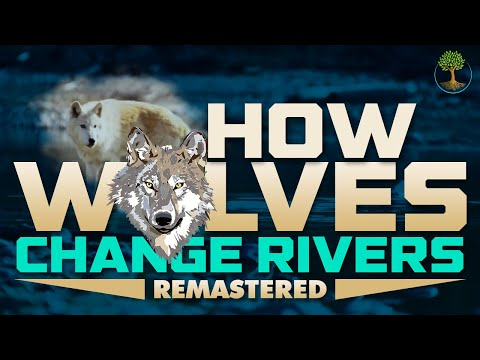
\includegraphics{index_files/mediabag/01234.jpg}}
\item
  \textbf{Simon Sinek: How Great Leaders Inspire Action}: A talk on the
  concept of ``Start With Why'' and inspiring leadership.
  \href{https://www.youtube.com/watch?v=qp0HIF3SfI4}{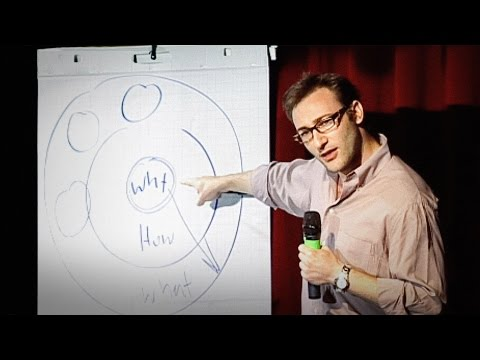
\includegraphics{index_files/mediabag/01.jpg}}
\item
  \textbf{RSA ANIMATE: Drive: The surprising truth about what motivates
  us}: An animated version of Dan Pink's talk on motivation.
  \href{https://www.youtube.com/watch?v=u6XAPnuFjJc}{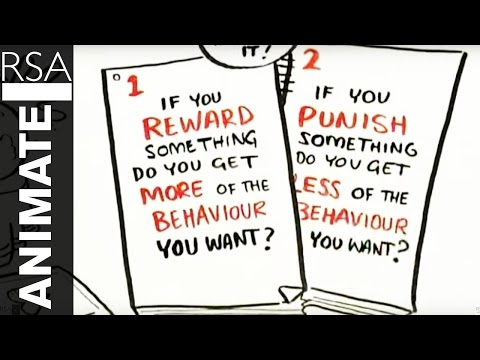
\includegraphics{index_files/mediabag/012.jpg}}
\item
  \textbf{The Power of Vulnerability - Brené Brown}: Research on
  vulnerability and its importance in fostering innovation.
  \href{https://www.youtube.com/watch?v=iCvmsMzlF7o}{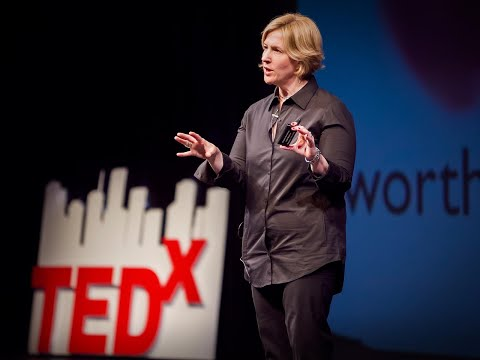
\includegraphics{index_files/mediabag/0123.jpg}}
\item
  \textbf{The Value of Supply Chain Management}: A comprehensive
  overview of the importance of supply chains in today's economy.
  \href{https://www.youtube.com/watch?v=9HD3C5vD3lU}{
\includegraphics{index_files/mediabag/012345.jpg}}
\item
  \textbf{The Power of Data in Supply Chains}: How data analytics is
  transforming the supply chain industry.
  \href{https://www.youtube.com/watch?v=U6YbVwX3v0Y}{
\includegraphics{index_files/mediabag/0123456.jpg}}
\item
  \textbf{Inside the Amazon Warehouse}: An inside look at the logistics
  and operations of Amazon's fulfillment centers.
  \href{https://www.youtube.com/watch?v=SzdbKz5CyhA}{
\includegraphics{index_files/mediabag/01234567.jpg}}
\item
  \textbf{The Future of AI in Supply Chain Management}: Exploring the
  potential of AI to revolutionize supply chains.
  \href{https://www.youtube.com/watch?v=2WjA8MsN9Bc}{
\includegraphics{index_files/mediabag/012345678.jpg}}
\end{itemize}

\section{Conclusion}\label{conclusion-6}

These resources are designed to support your journey in the Value Chain
Hackers program. By utilizing these tools, platforms, reading materials,
and videos, you'll be well-equipped to tackle the challenges and
opportunities in supply chain management. Let's make the most of these
resources to innovate and drive impactful change in the supply chain
industry!

\bookmarksetup{startatroot}

\chapter{Summary}\label{summary}

\bookmarksetup{startatroot}

\chapter{Summary}\label{summary-1}

\section{Reflecting on Our Journey 🚀}\label{reflecting-on-our-journey}

As we come to the end of this onboarding documentation, let's take a
moment to reflect on the journey ahead with the Value Chain Hackers
program. This program is designed to equip you with the skills,
knowledge, and resources needed to make a significant impact in the
field of supply chain management.

\section{Key Takeaways}\label{key-takeaways}

\subsection{Embracing Innovation 🌟}\label{embracing-innovation}

At the heart of Value Chain Hackers is a commitment to innovation. We
leverage cutting-edge tools, methodologies, and technologies to tackle
real-world supply chain challenges. From AI integration to Agile-Scrum
methodologies, we are always pushing the boundaries of what's possible.

\subsection{Collaborative Learning 🤝}\label{collaborative-learning}

Collaboration is a cornerstone of our approach. By working closely with
peers, mentors, and industry experts, you'll gain diverse perspectives
and insights. Our digital lab ensures that collaboration happens
seamlessly, no matter where you are.

\subsection{Real-World Impact 🌍}\label{real-world-impact-1}

Every project you undertake here is designed to have a real-world
impact. You'll be working on practical problems, developing solutions
that can be implemented in the industry. This hands-on experience is
invaluable in preparing you for your future career.

\subsection{Continuous Improvement 🔄}\label{continuous-improvement-3}

The Agile-Scrum framework emphasizes continuous improvement. Through
regular feedback, retrospectives, and iterative development, you'll
constantly refine your skills and solutions. This mindset of continuous
learning and adaptation is crucial in today's fast-paced world.

\subsection{Community and Support 🧑‍🤝‍🧑}\label{community-and-support}

You are not alone in this journey. The Value Chain Hackers community is
here to support you every step of the way. From mentors providing
guidance to peers offering collaboration, you have a network that is
dedicated to your success.

\section{Next Steps}\label{next-steps}

\begin{enumerate}
\def\labelenumi{\arabic{enumi}.}
\tightlist
\item
  \textbf{Engage with the Community}: Join our communication channels on
  Discord and stay connected with your peers and mentors.
\item
  \textbf{Dive into Projects}: Start working on your assigned projects,
  using the tools and resources provided to make meaningful progress.
\item
  \textbf{Seek Feedback}: Regularly engage with your mentors and peers
  for feedback and insights to improve your work.
\item
  \textbf{Participate Actively}: Take part in all scheduled activities,
  from SCRUM meetings to hackathons, to make the most of this learning
  experience.
\item
  \textbf{Reflect and Improve}: Use retrospectives and feedback sessions
  to reflect on your progress and identify areas for improvement.
\end{enumerate}

\section{Final Thoughts}\label{final-thoughts}

The Value Chain Hackers program is more than just a learning experience;
it's an opportunity to make a difference. By harnessing the power of
collaboration, innovation, and continuous improvement, you'll develop
solutions that can transform the supply chain industry. We're excited to
see the amazing things you'll achieve and the impact you'll make.

Welcome aboard, and let's hack the value chain together!

Christiaan Verhoef Value Chain Hackers Leader

\bookmarksetup{startatroot}

\chapter{Presentations}\label{presentations}

\subsection{13-06-2024 planning}\label{planning}

\begin{itemize}
\tightlist
\item
  \textbf{Date:} june 13, 2024
\item
  \textbf{Description:} This presentation coveres the \textbf{planning}
  to do the first infrastructure launch
\item
  \href{./13-05-2024\%20planning.qmd}{View Slides}
\end{itemize}

\subsection{30-05-2024 Planning}\label{planning-1}

\begin{itemize}
\tightlist
\item
  \textbf{Date:} May 30, 2024
\item
  \textbf{Description:} planning from Sprint 1 with sebastien
\item
  \href{./30-05-2024\%20Planning.html}{View Slides}
\end{itemize}

\subsection{22-05-2024 presentation}\label{presentation}

\begin{itemize}
\tightlist
\item
  \textbf{Date:} May 30, 2024
\item
  \textbf{Description:} This presentation covers the planning phase for
  our upcoming projects.
\item
  \href{./22-05-2024\%20presentation2.qmd}{View Slides}
\end{itemize}

\begin{Shaded}
\begin{Highlighting}[]
\NormalTok{graph TD}
\NormalTok{style Requirements fill:\#ffa500, stroke:\#000000}
\NormalTok{style Backlog fill:\#ffff00, stroke:\#000000}
\NormalTok{style SprintPlanning fill:\#ffa500, stroke:\#000000}
\NormalTok{style Sprint fill:\#008000, stroke:\#000000}
\NormalTok{style DailyScrum fill:\#ffa500, stroke:\#000000}
\NormalTok{style Development fill:\#008000, stroke:\#000000}
\NormalTok{style Testing fill:\#008000, stroke:\#000000}
\NormalTok{style Review fill:\#ffa500, stroke:\#000000}
\NormalTok{style Retrospective fill:\#ffa500, stroke:\#000000}
\NormalTok{style ProductRelease fill:\#ff0000, stroke:\#000000}

\NormalTok{subgraph AgileDevelopment}
\NormalTok{    Requirements[Requirements] {-}{-}\textgreater{} Backlog[Product Backlog]}
\NormalTok{    Backlog {-}{-}\textgreater{} SprintPlanning[Sprint Planning]}
\NormalTok{    SprintPlanning {-}{-}\textgreater{} Sprint[Sprint]}
\NormalTok{    Sprint {-}{-}\textgreater{} DailyScrum[Daily Scrum]}
\NormalTok{    Sprint {-}{-}\textgreater{} Development[Development]}
\NormalTok{    Development {-}{-}\textgreater{} Testing[Testing]}
\NormalTok{    Testing {-}{-}\textgreater{} Review[Sprint Review]}
\NormalTok{    Review {-}{-}\textgreater{} Retrospective[Sprint Retrospective]}
\NormalTok{    Retrospective {-}{-}\textgreater{} Backlog}
\NormalTok{    Review {-}{-}\textgreater{} ProductRelease[Product Release]}
\NormalTok{end}
\end{Highlighting}
\end{Shaded}

\bookmarksetup{startatroot}

\chapter{References}\label{references}

\bookmarksetup{startatroot}

\chapter{References}\label{references-1}

Lorem ipsum dolor sit amet, consectetur adipiscing elit. Sed do eiusmod
tempor incididunt ut labore et dolore magna aliqua.



\end{document}
